\begin{figure}[H]
\centering
\begin{subfigure}[b]{.49\textwidth}
    \centering
    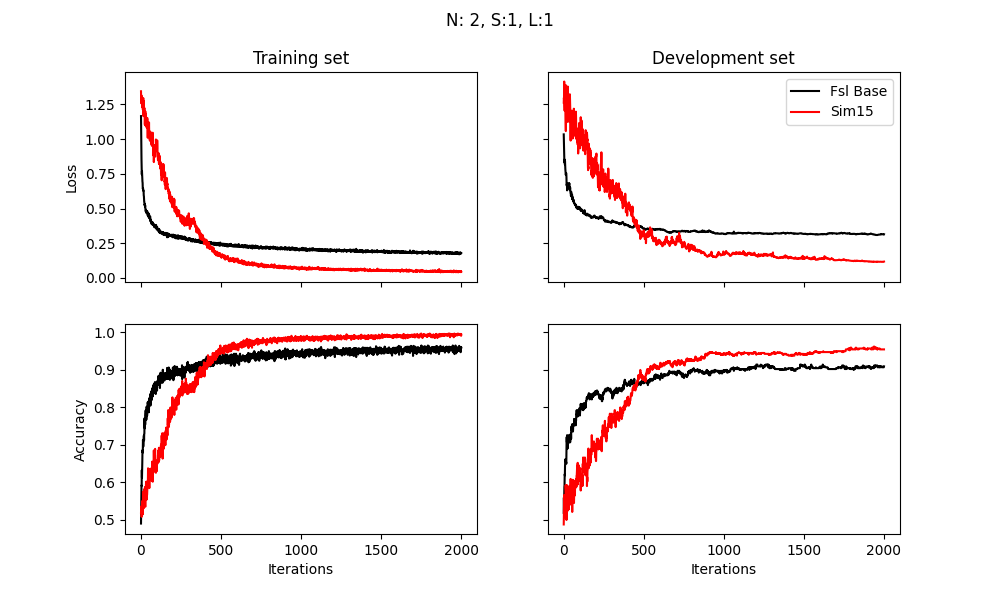
\includegraphics[width=\textwidth]{figures/comparison/Epochs_2000--A_0.05--N_2--S_1--L_1.png}
\end{subfigure}
\begin{subfigure}[b]{.49\textwidth}
    \centering
    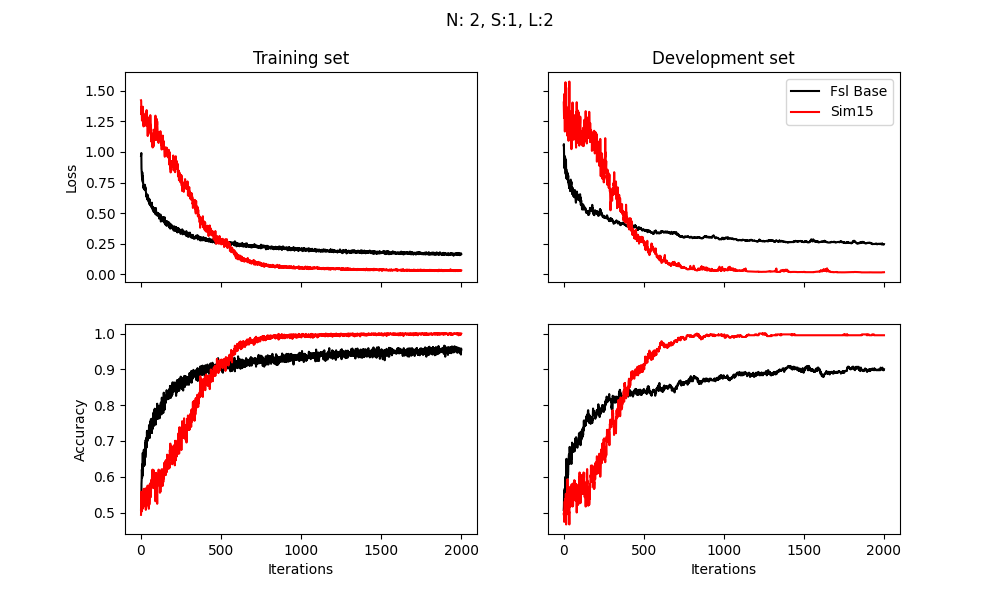
\includegraphics[width=\textwidth]{figures/comparison/Epochs_2000--A_0.05--N_2--S_1--L_2.png}
\end{subfigure}
\begin{subfigure}[b]{.49\textwidth}
    \centering
    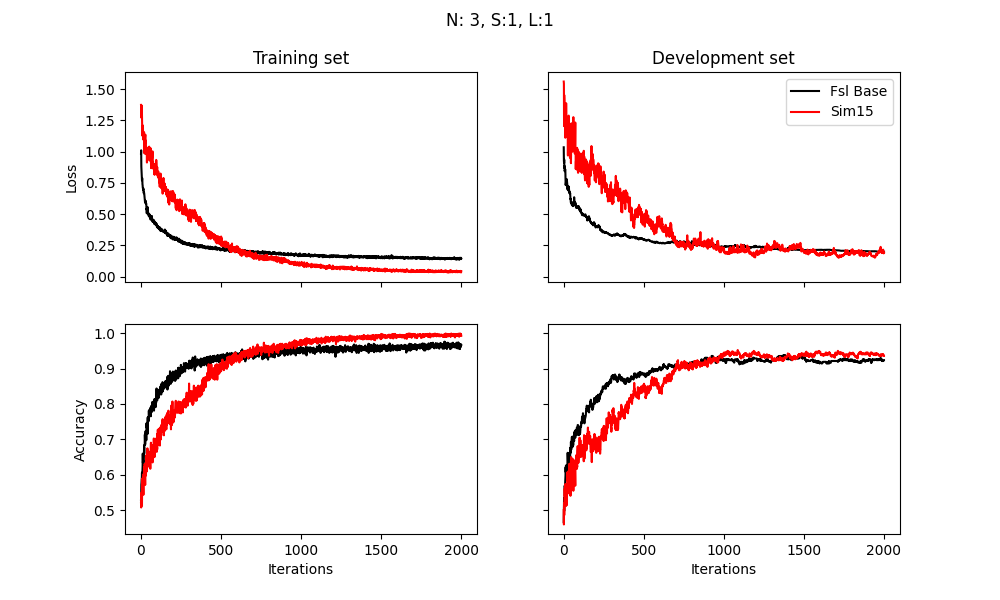
\includegraphics[width=\textwidth]{figures/comparison/Epochs_2000--A_0.05--N_3--S_1--L_1.png}
\end{subfigure}
\begin{subfigure}[b]{.49\textwidth}
    \centering
    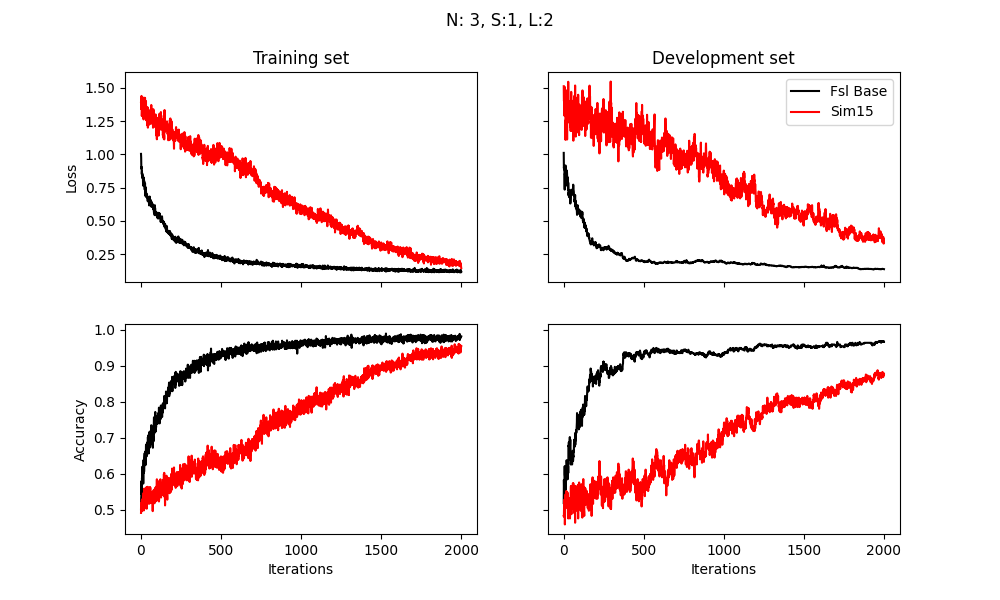
\includegraphics[width=\textwidth]{figures/comparison/Epochs_2000--A_0.05--N_3--S_1--L_2.png}
\end{subfigure}
\begin{subfigure}[b]{.49\textwidth}
    \centering
    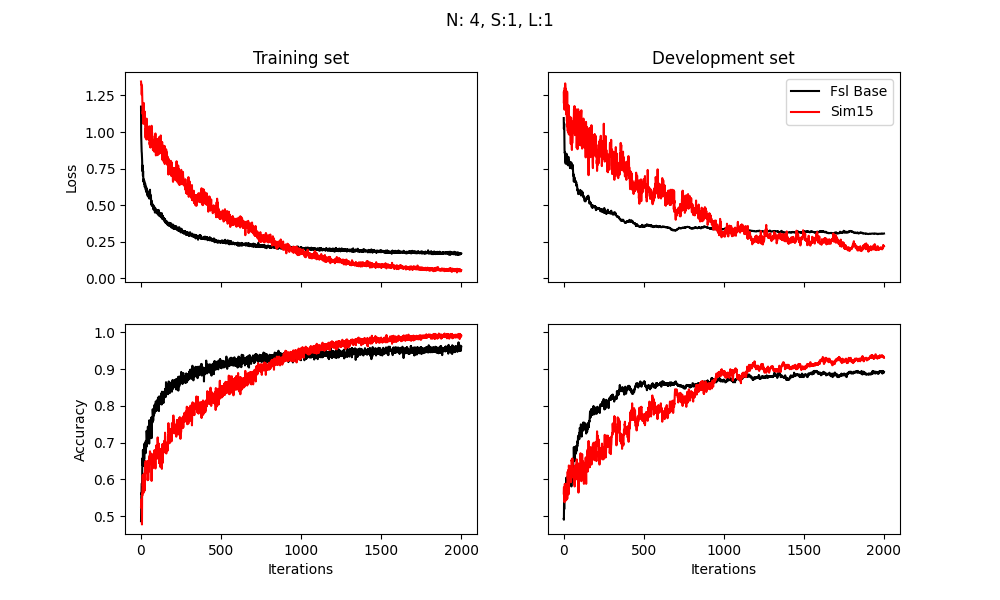
\includegraphics[width=\textwidth]{figures/comparison/Epochs_2000--A_0.05--N_4--S_1--L_1.png}
\end{subfigure}
\begin{subfigure}[b]{.49\textwidth}
    \centering
    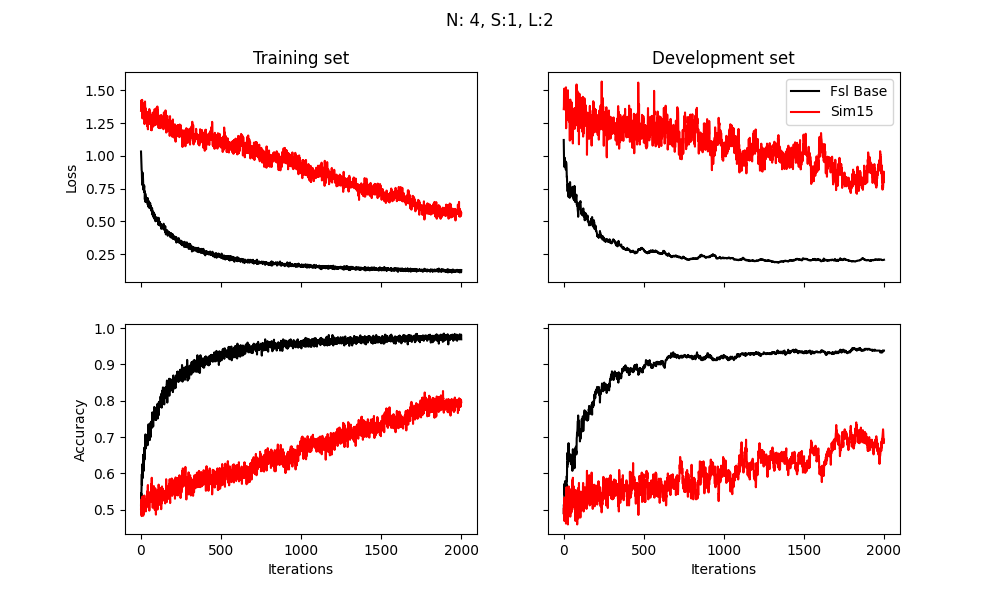
\includegraphics[width=\textwidth]{figures/comparison/Epochs_2000--A_0.05--N_4--S_1--L_2.png}
\end{subfigure}\\
\begin{subfigure}[b]{\textwidth}
    \raggedright
    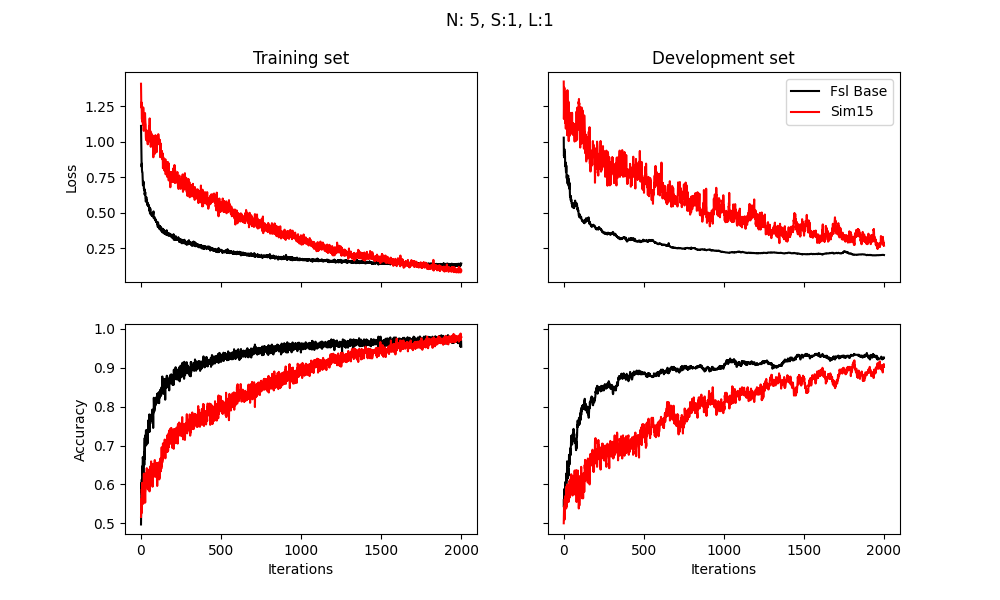
\includegraphics[width=0.5\textwidth]{figures/comparison/Epochs_2000--A_0.05--N_5--S_1--L_1.png}
\end{subfigure}
\caption[Comparison between two \mya]{\label{fig:test1}Training behaviour for two types of \mya on the MC task after 2000 training Epochs.}
\end{figure}